\documentclass[tikz,border=3pt]{standalone}
\usepackage[utf8]{inputenc}
\usepackage[T1]{fontenc}
\usepackage{lmodern}
\renewcommand{\familydefault}{\sfdefault}
\usepackage{sansmath}\sansmath
\usepackage{chemfig}
\usepackage{pgfplots}\pgfplotsset{compat=1.18,/pgf/number format/use comma,/pgf/number format/1000 sep={.}}
\usetikzlibrary{arrows.meta,calc,positioning,decorations.pathmorphing,patterns}
% paleta del sitio
\definecolor{nar}{HTML}{E8680C}\definecolor{narc}{HTML}{FFB35C}\definecolor{hielo}{HTML}{FFF3E8}
\definecolor{tinta}{HTML}{1D1D1F}\definecolor{gris}{HTML}{6E6E73}\definecolor{lila}{HTML}{7C5CF0}
\definecolor{azul}{HTML}{2F6FD6}\definecolor{menta}{HTML}{17A673}\definecolor{coral}{HTML}{E8342A}
\begin{document}
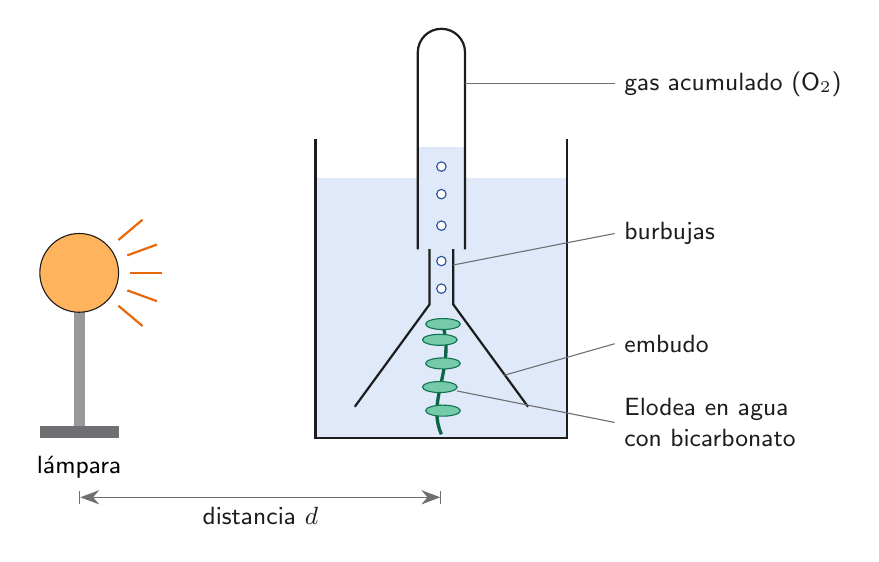
\begin{tikzpicture}[font=\small,>={Stealth[length=2.4mm]}]
% lámpara
\fill[gris] (-0.5,0) rectangle (0.5,0.15); \fill[gris!70] (-0.07,0.15) rectangle (0.07,1.6);
\draw[tinta,fill=narc] (0,2.1) circle (0.5);
\foreach \a in {-40,-20,0,20,40} \draw[nar,thick] ($(0,2.1)+(\a:0.65)$) -- ($(0,2.1)+(\a:1.05)$);
\node[anchor=north] at (0,-0.1) {lámpara};
% vaso
\fill[azul!15] (3,0) rectangle (6.2,3.3);
\draw[tinta,thick] (3,3.8) -- (3,0) -- (6.2,0) -- (6.2,3.8);
% elodea
\draw[menta!60!black,very thick] (4.6,0.05) .. controls (4.4,0.5) and (4.8,0.9) .. (4.6,1.5);
\foreach \y/\s in {0.35/1,0.65/-1,0.95/1,1.25/-1,1.45/1} \draw[menta!70!black,fill=menta!60] (4.6+0.02*\s,\y) ellipse ({0.22} and 0.07);
% embudo invertido
\draw[tinta,thick] (3.5,0.4) -- (4.45,1.7) -- (4.45,2.6);
\draw[tinta,thick] (5.7,0.4) -- (4.75,1.7) -- (4.75,2.6);
% tubo de ensayo invertido
\fill[white] (4.3,2.9) rectangle (4.9,4.9); \fill[white] (4.6,4.9) circle (0.3);
\fill[azul!15] (4.3,2.4) rectangle (4.9,3.7);
\draw[tinta,thick] (4.3,2.4) -- (4.3,4.9) arc (180:0:0.3) -- (4.9,2.4);
\foreach \y in {1.9,2.25,2.7,3.1,3.45} \draw[azul!70!black,fill=white] (4.6,\y) circle (0.06);
\draw[gris] (4.9,4.5) -- (6.8,4.5) node[anchor=west,text=tinta,align=left] {gas acumulado (O$_2$)};
\draw[gris] (4.75,2.2) -- (6.8,2.6) node[anchor=west,text=tinta,align=left] {burbujas};
\draw[gris] (5.4,0.8) -- (6.8,1.2) node[anchor=west,text=tinta,align=left] {embudo};
\draw[gris] (4.8,0.6) -- (6.8,0.2) node[anchor=west,text=tinta,align=left] {Elodea en agua\\con bicarbonato};
% distancia
\draw[gris,|<->|] (0,-0.75) -- (4.6,-0.75) node[midway,below,text=tinta] {distancia $d$};
\end{tikzpicture}
\end{document}
